\documentclass[a4paper,10pt]{scrartcl}

\usepackage{standalone}

% Load ``float'' before ``hyperref`` before ''algorithm``
% Note: ''algorithm`` would load ''float`` by itself
\usepackage{float}
\usepackage[pagebackref,hyperindex=true]{hyperref}

%%%%%%%%%%%%%%%%%%%%%%%%%%%%
% Math
%%%%%%%%%%%%%%%%%%%%%%%%%%%%
\usepackage{amsmath}
\usepackage{amssymb}
\usepackage{amsfonts}
\usepackage{amsopn}
\usepackage{braket}
\usepackage{bbm}
\usepackage{dsfont}
% \usepackage{mathabx}


% Various new commands that ease typesetting math even further
% \newcommand{\assign}{\ensuremath{\coloneq}}
% \newcommand{\rassign}{\ensuremath{\eqcolon}}
% TODO: remove
% \newcommand{\assign}{\ensuremath{:=}}
% \newcommand{\rassign}{\ensuremath{=:}}
% \newcommand{\seteq}{\ensuremath{\overset{!}{=}}}
% \newcommand{\of}[1]{\ensuremath{\left( #1 \right)}}
% \newcommand{\ofs}[1]{\ensuremath{\left( #1 \right)}}
% \newcommand{\norm}[1]{\ensuremath{\| #1 \|}}
% \newcommand{\tmop}[1]{\ensuremath{\operatorname{#1}}}
% \newcommand{\id}{\ensuremath{\mathds{1}}}
% % \newcommand{\id}{\ensuremath{I}}
% \newcommand{\kron}[1]{\ensuremath{\delta_{#1}}}
% \newcommand{\conj}[1]{\ensuremath{\overline{#1}}}
% \renewcommand{\vec}[1]{\ensuremath{\underline{#1}}}
% \newcommand{\mat}[1]{\ensuremath{\mathbf{#1}}}
% \newcommand{\inv}{\ensuremath{{}^{-1}}}
% \newcommand{\T}{\ensuremath{{}^{\textnormal{T}}}}
% \renewcommand{\H}{\ensuremath{{}^{\textnormal{H}}}}
% \newcommand{\Tinv}{\ensuremath{{}^{\textnormal{-T}}}}
% \newcommand{\Hinv}{\ensuremath{{}^{\textnormal{-H}}}}
% \newcommand{\tr}{\ensuremath{\textnormal{Tr}}}
% \newcommand{\ft}[1]{\ensuremath{\mathcal{F}\left(#1\right)}}
% \newcommand{\ift}[1]{\ensuremath{\mathcal{F}^{-1}\left(#1\right)}}
% \newcommand{\fft}[1]{\ensuremath{\mathtt{FFT}\left(#1\right)}}
% \newcommand{\ifft}[1]{\ensuremath{\mathtt{IFFT}\left(#1\right)}}
% \newcommand{\dotp}[2]{\ensuremath{\left\langle #1 , #2 \right\rangle}}
% \newcommand{\bigO}[1]{\ensuremath{\mathcal{O}\left( #1 \right)}}
% \newcommand{\laplace}{\ensuremath{\operatorname{\Delta}}}
% \newcommand{\diff}[3][]{\frac{\mathrm{d}^{#1}#2}{\mathrm{d}#3^{#1}}}
% \newcommand{\pdiff}[3][]{\frac{\partial^{#1}#2}{\partial #3^{#1}}}

%%%%%%%%%%%%%%%%%%%%%%%%%%%%
% Graphics
%%%%%%%%%%%%%%%%%%%%%%%%%%%%
\usepackage{graphicx}
\usepackage{subfig}
\usepackage{asymptote}
\usepackage{tikz}
\usetikzlibrary{topaths,calc}
\usetikzlibrary{positioning}
\usetikzlibrary{arrows,shapes,backgrounds}
\definecolor{gray}{gray}{0.55}


%%%%%%%%%%%%%%%%%%%%%%%%%%%%
% Math
%%%%%%%%%%%%%%%%%%%%%%%%%%%%
\usepackage{algorithm}
% \usepackage{algorithmic}
\usepackage{color}
\usepackage{relsize}
\usepackage[scaled=0.8]{beramono}

%%%%%%%%%%%%%%%%%%%%%%%%%%%%
% Code
%%%%%%%%%%%%%%%%%%%%%%%%%%%%
\usepackage{listings}
% C++ Code macro
\newcommand{\cpp}[1] {
  \lstset{language=c++,
          basicstyle=\smaller,
          basewidth=0.58em,
          columns=fixed,
          tabsize=2,
          fontadjust=true,
          frame=l,
          xleftmargin=4.2pt,
          numbers=left,
          stepnumber=2,
          breaklines=true,
          breakindent=0pt,
          prebreak=\mbox{\tiny$\searrow$},
          postbreak=\mbox{{\color{gray}$\cdots$}},
          numberstyle=\color{gray},
          commentstyle=\color{gray},
          stringstyle=\textit,
          showstringspaces=false,
        }
  \lstinputlisting{#1}
}
  
  \lstset{language=c++,
          basicstyle=\smaller,
          basewidth=0.58em,
          columns=fixed,
          tabsize=2,
          fontadjust=true,
          breaklines=true,
          breakindent=0pt,
          prebreak=\mbox{\tiny$\searrow$},
          postbreak=\mbox{{\color{gray}$\cdots$}},
          numberstyle=\color{gray},
          commentstyle=\color{gray},
          stringstyle=\textit,
          showstringspaces=false,
          basicstyle=\footnotesize
        }


%%%%%%%%%%%%%%%%%%%%%%%%%%%%
% More Packages
%%%%%%%%%%%%%%%%%%%%%%%%%%%%
\usepackage[utf8x]{inputenc}
\usepackage{cancel}
\usepackage{url}
\usepackage{placeins}
\usepackage{microtype}
\usepackage{amsthm}
\newtheorem{theorem}{Theorem}
\newtheorem{definition}{Definition}

% Links in pdf
\usepackage{color}
\newcommand{\blue}{ \color{blue} }
\definecolor{linkcol}{rgb}{0,0,0.4}
\definecolor{citecol}{rgb}{0.5,0,0}

\hypersetup
{
colorlinks=true,
linkcolor=linkcol,
citecolor=citecol,
urlcolor=linkcol
}

% nicer backref links
\renewcommand*{\backref}[1]{}
\renewcommand*{\backrefalt}[4]{%
\ifcase #1 %
(Not cited.)%
\or
(Cited on page~#2.)%
\else
(Cited on pages~#2.)%
\fi}
\renewcommand*{\backrefsep}{, }
\renewcommand*{\backreftwosep}{ and~}
\renewcommand*{\backreflastsep}{ and~}

% TODO: set some indent
% \parindent 0cm

\newcommand{\clearemptydoublepage}{\newpage{\pagestyle{empty}\cleardoublepage}}


% Mycommands

\usepackage{bm}

% \newcommand*{\op}[1]{\hat{\mathcal{#1}}}
\newcommand*{\C}{\ensuremath{\mathbb{C}}}
\newcommand*{\Dt}{\ensuremath{\Delta t}}
\newcommand*{\K}{\ensuremath{\mathfrak{K}}}
\newcommand*{\R}{\ensuremath{\mathbb{R}}}
\newcommand*{\bmat}[1]{\bm{#1}}
\newcommand*{\bvec}[1]{\bm{#1}}
\newcommand*{\conj}[1]{\overline{#1}}
\newcommand*{\del}{\ensuremath{\partial}}
\newcommand*{\dif}{\ensuremath{d}}
\newcommand*{\dt}{\ensuremath{\delta t}}
\newcommand*{\eps}{\ensuremath{\varepsilon}}
\newcommand*{\im}{\ensuremath{\imath}}
\newcommand*{\opH}{\mathcal{H}}
\newcommand*{\opT}{\mathcal{T}}
\newcommand*{\opU}{\mathcal{U}}
\newcommand*{\opV}{\mathcal{V}}
\newcommand*{\opW}{\mathcal{W}}
\newcommand*{\opA}{\mathcal{A}}
\newcommand*{\opB}{\mathcal{B}}
\newcommand*{\opX}{\mathcal{X}}
\newcommand*{\upic}{\ensuremath{u[\Pi,\bm{c}]}}
\newcommand*{\proc}[1]{\textsc{#1}}

\usepackage{algorithm}
\usepackage{verbatim}
\usepackage{physics}
\usepackage{amssymb}
\usepackage{bm}
% \usepackage[noend]{algpseudocode}
\usepackage{algpseudocode}


\usepackage{tikz}
\usetikzlibrary{arrows,chains,matrix,positioning,scopes}
\usepackage{multicol}





\usepackage{tikz}
\usetikzlibrary{arrows,chains,matrix,positioning,scopes}







\begin{document}

\begin{titlepage}
\begin{center}
  \hfill
  \vspace{3.0cm}

  {\huge \textsc{Spawning of wave-packets in 1D non-adiabatic transitions\\[10pt]
  }}
  ~\\[20pt]

  {\huge{Term Thesis}}\\[2.5cm]

  {\emph{written by}}\\
  Raoul Bourquin
  \\[0.6cm]
  {\emph{supervised by}}\\
  Dr. Vasile Gr\u{a}dinaru\\
  {\emph{and}}\\
  Prof. Dr. Ralf Hiptmair
  \\[2.5cm]

  Seminar for Applied Mathematics\\
  ETH Zurich
  \\[0.5cm]
  \emph{{Spring semester 2011}}
\end{center}
\end{titlepage}

\clearemptydoublepage

\mbox{}
\vfill
\begin{abstract}
	This article explains the central design decisions and most important code details related to the efficient implementation of time propagation for Hagedorn quantum wave packets in the WaveBlocks framework.
	A short introduction to operator splitting and a summary of some of the most important time propagation schemes for quantum wave packets are also given.
	Finally, some benchmarking results are presented in the context of an example of a ???Ddim Nlevel BLUB potential???.
\end{abstract}

\vfill
\tableofcontents

\clearpage

\listoffigures
\listofalgorithms

\clearemptydoublepage \chapter{Introduction}

\section{Motivation}
To test the reliability of a numerical method or an approximation, e.g. such as in \cite{B_bachelor_thesis}, an implementation in python is sufficient. Python is easy to understand and the code can also be used as a base e.g. for a C++ version. A python framework to solve the time-dependent Schr\"odinger equation with a semiclassical approach with \textit{Hagedorn} wavepackets is already availabla on github \cite{waveblocksnd}. This can be used for example to test different propagation schemes, integration methods or integration partitions. In case longer simulations or solving higher dimensional problems is desired the execution time could increase rapidly in a python implementation. Therefore it is necessary to port the python implementation to C or C++ which are highly time efficient. The core implementation is already available in C++ on github \cite{libwaveblocks} but further improvement is desired. This implementation currently uses an external project \cite{eigen3-hdf5} for writing data in HDF5 format. This project is sufficient if the user supervises the generated data. The goal of this project is to use the HDF5 interface \cite{hdf5cppdoc} directly to write data in a comparable way to python. This further allows to implement a data test which can compare data files between python and C++. This was done with the well-known \textit{GoogleTest} \cite{googletest} framework.

\section{Background}
\label{seq:background}

In quantum physics the most prominent problems are governed by the time-dependent
Schr\"odinger equation \ref{eq:basics_tdse_simple}

\begin{equation} \label{eq:basics_tdse_simple}
  i \hbar \frac{\partial}{\partial t} \Ket{\psi} = H \Ket{\psi}
\end{equation}

where $H$ is the Hamiltonian, $\psi(x,t)$ represents the wave function dependent on position $x$ and
time $t$ and $\langle \psi | \psi  \rangle$ is the probability density of electrons. This can be found in the most basic courses and books about quantum physics. This equation can be reformulated in a semiclassical setting for nuclei as: \
\begin{equation}
\label{eq:tdse_sc_nuclei}
 i\hbar \partial_{t}\psi = \left( -\frac{\hbar^{2}}{2} \Delta_{x} + V(\vec{x}) \right) \psi\,.
\end{equation}

The goal is to search for $\psi = \psi(\vec{x},t)$ depending on the spatial variables $\vec{x} = (x_{1},\ldots,x_{d}) \in \mathbb{R}^{d}$ and the time $t\in \mathbb{R}$. In this context $\Delta_{x}$ is the Laplace operator and $V$ is a smooth real-valued potential $V$, e.g. an electronic energy surface in the time-dependent Born-Oppenheimer approximation. Nevertheless there are still much challenges involved to solve this equation \ref{eq:tdse_sc_nuclei}. One of this is the high dimensionality of this equation. A molecule with $N$ nuclei where each of them has three degrees of freedom results in $3N$ unknowns. For example the simple molecule $\mathrm{CO_{2}}$ has already $d=9$ degrees of freedom. Another challenge is the multiple scales governed by the small parameter $\hbar = \varepsilon^{2}$ in case of $\mathrm{CO_{2}}$ it results in $\hbar \approx 0.0058$. Also the actual solution has frequencies of order $1/\hbar$ which are hard to reproduce for small $\hbar$ on a finite uniform grid as required by a Fourier based approach. Further there is the problem of long time evolutions.\\

An additional method is to use raising and lowering operators for semiclassical wavepackets \cite{H_ladder_operators}. The raising and lowering operators $\mathcal{R}$ and $\mathcal{L}$ produce a complete $L^2$-orthonormal set of basis functions $\phi_{\vec{k}}(\vec{x}) = \phi_{\vec{k}}^\hbar[\vec{q},\vec{p},\mat{Q},\mat{P}](\vec{x})$ (for multi-indices $\vec{k} = (k_1,\dots,k_d)$ with non-negative integers $k_j$) obeying the three-term recurrence:
\begin{equation*}
          \left(\sqrt{k_{j}+1}\phi_{\vec{k}+\vec{e^j}}\right)_{j=1}^{d}
          = \sqrt{\frac{2}{\hbar}} \mat{Q}\inv \left(\vec{x}-\vec{q}\right) \phi_{\vec{k}} -
          \mat{Q}\inv \conj{\mat{Q}} \left(\sqrt{k_{j}} \phi_{\vec{k}-\vec{e^j}}\right)_{j=1}^{d}
\end{equation*}

Therefore we can have Hagedorn wavepackets of the following form:
        \begin{equation*}
          \begin{split}
            \phi_{\vec{0}}^\hbar & [\vec{q},\vec{p},\mat{Q},\mat{P}](\vec{x})\ =
            (\pi\hbar)^{-\frac{d}{4}} (\det \mat{Q})^{-\frac{1}{2}} \,\times \\
            & \exp\left(\frac{i}{2\hbar} \left(\vec{x}-\vec{q}\right)\T \mat{P}\mat{Q}\inv \left(\vec{x}-\vec{q}\right) +
              \frac{i}{\hbar} \vec{p}\T \left(\vec{x}-\vec{q}\right) \right)
          \end{split}
        \end{equation*}
where $\vec{q}\in \mathbb{R}^d$ and $\vec{p}\in \mathbb{R}^d$ represent the position and momentum, respectively, and $\mat{Q}$ and $\mat{P}$ are complex $d\times d$ matrices satisfying some compatibility relations. For detailed explanation see \cite{FGL_semiclassical_dynamics}. In there is also a basic time propagation algorithm described. Further improvement and proof was presented in \cite{GH_convsemiclassical} about convergence of semiclassical wavepackets based time-splitting.\\

This methods were implemented by Raoul Bourquin as master thesis \cite{B_master_thesis} in python and is available on github \cite{waveblocksnd}. This code can be used in applications e.g tunneling dynamics and spawning \cite{GHJ_tunneling_spawning} or non-adiabatic transition near avoided crossing \cite{BGH_natac}. Until now only the core of this implementation was also already ported to C++. Hagedorn wavepackets was done by Michaja B\"osch \cite{bt_michajab}, inner products and quadrature by Benedek Vartok \cite{st_benedekv} and matrix potentials by Lionel Miserez \cite{bt_lionelm}. This core implementation is available on github \cite{libwaveblocks}. In this project the goal was to enlarge the C++ code functionality with intelligent data serialization. The goal was to reach compatibility between the python and C++ implementation on how data is stored using the \textit{HDF5} interface. This further allowed to use the \textit{GoogleTest} framework to write a data test for the two \textit{HDF5} files. This can be convenient because now we can test if both implementation generate the same data or if there could be a bug in the code.
\clearpage \section{Operator Splitting for Time Propagation}
\label{sec:operatorsplitting}
%
In this report, we will use the variable $D$ for describing the number of dimensions and $N$ for the number of energy levels in the system.
The semiclassical time-dependent Schrödinger equation is of the form
%
\begin{align}
	\label{math:tdse}
	\im \eps \; \del_t \psi (\bvec{x},t) = \opH (\eps) \; \psi (\bvec{x},t)
\end{align}
%
with Hamiltonian operator $\opH$, wave function $\psi(\bvec{x},t)$ depending on the spatial variables $\bvec{x} = (x_1,\dots,x_D) \in \R^D$ and the time variable $t \in \R$.
The parameter $\eps$, also known as the semiclassical parameter, determines the degree of influence of quantum dynamics, approaching classical dynamics in the limit $\eps \rightarrow 0$ and full quantum mechanics for $\eps = 1$. \\
Moreover, $\eps$ plays an important role in the stability of numerical schemes.
As underlined in \cite{GH_convsemiclassical}, a small parameter $\eps$ can often impose severe constraints on the step size of splitting methods and significantly increase the error. For example, the error was shown to be proportional to $\eps^{-2}$ for Lie-Trotter splitting, Strang splitting and other related methods, meaning that smaller $\eps$ would lead to a larger error.
\par\medskip
%
The solution to the above Schrödinger equation \ref{math:tdse} can be approximated as a finite linear combination of Hagedorn functions 
\begin{align}
	\label{math:hagedornwp}
	\psi(\bvec{x},t) \approx u(\bvec{x},t)
	= e^{\im S(t)/\eps^2} \sum_{k \in \K} c_k(t) \varphi_k^\eps [ \bvec{\Pi} (t) ] (\bvec{x})
\end{align}
where $\K$ represents a finite multi-index set, $c_k \in \C$ are coefficients that depend on time only, $S(t)$ is a phase factor and $\bvec{q},\bvec{p} \in \R^D$ and $\bmat{Q},\bmat{P} \in \C^{D \times D}$ are some parameters.
For convenience, the notation for the parameter pack $\bvec{\Pi} (t) = (\bvec{q}(t),\bvec{p}(t),\bvec{Q}(t),\bvec{P}(t))$ is introduced.
It is worth noting that $\varphi_k^\eps [ \bvec{\Pi} (t) ]$ depends on time $t$ only implicitly through the time dependency of $\bvec{q}(t),\bvec{p}(t),\bvec{Q}(t),\bvec{P}(t)$.
A more detailed analysis of Hagedorn functions is given in \cite{FGL_semiclassical_dynamics} and a comprehensive overview over the relevant mathematical details can be found in \cite{B_master_thesis}.
\par\medskip
%
The Schrödinger equation \ref{math:tdse} can be solved using the ansatz
\begin{align}
	\psi (\bvec{x},t+dt) = \exp \left( - \frac{\im}{\eps^2} \opH t \right) \; \psi (\bvec{x},t) \; .
\end{align}
%
This matrix exponential is very expensive to compute.
Instead, in the search for a numerical solution, one can exploit the structure of the Hamiltonian operator $\opH$, by splitting it into its kinetic part $\opT$ and potential part $\opV$.
Furthermore, for the rest of this report we will denote by $\opU$ and $\opW$ the quadratic and non-quadratic component of $\opV$ respectively and it will be used that
%
\begin{align}
	\opV &= V(\bvec{x}) \\ 
	\opU &= U(\bvec{q},\bvec{x}) := V(\bvec{q}) + \nabla V(\bvec{q}) (\bvec{x}-\bvec{q})
	+ \frac{1}{2} (\bvec{x}-\bvec{q})^T \nabla^2 V(\bvec{q}) (\bvec{x}-\bvec{q}) \\
	\opW &= W(\bvec{q},\bvec{x}) := V(\bvec{x}) - U(\bvec{q},\bvec{x})
\end{align}
%
In other words, $\opU = U(\bvec{q},\bvec{x})$ is the second order Taylor expansion of the potential energy $\opV = V(\bvec{x})$ around $\bvec{q}$ (the coordinate $\bvec{q}$ will be omitted for simplicity of notation) and $\opW = W(\bvec{q},\bvec{x})$ is the corresponding remainder.
\par\medskip
%
By further recalling the form of the kinetic operator $\opT$ (for a particle of mass $m=1$)
\begin{align}
	\opT &= - \sum_{j=1}^D \frac{\eps^4}{2} \frac{\del^2}{\del x_j^2}
\end{align}
%
one can then split the Hamiltonian operator $\opH$ into the components
%
\begin{align}
	\opH = \opT + \opV = \opT + \opU + \opW
\end{align}
%
This splitting is so central to the construction of the time propagators in the following sections that it is worthwhile repeating the most important findings from \cite{FGL_semiclassical_dynamics}:
\begin{itemize}
	\item The free particle Schrödinger equation ($\opV=0$) can be solved exactly and the wave packet remains in Hagedorn wave packet form (equation~\ref{math:hagedornwp}).
		For time propagation, only the parameters $\bvec{\Pi},S$ need to be updated, the coefficients $\{c_k\}_{k \in \K}$ remain unchanged.
	\item The Schrödinger equation~\ref{math:tdse} can be solved exactly in a pure quadratic potential, i.e. in a potential $\opV=U(\bvec{x})$ with $\opT=0$.
		Again, time propagation only affects the parameters $\bvec{\Pi},S$, not the coefficients $\{c_k\}_{k \in \K}$.
	\item In the case of an arbitrary potential $\opV = W(\bvec{x})$ that is not quadratic, a variational approach can be used.
		A set of Galerkin functions can be propagated by adapting the coefficients $\{c_k\}_{k \in \K}$ without changing the parameters $\bvec{\Pi},S$.
\end{itemize}
%
The following sections will heavily make use of these properties in order to build composition methods for time integration of quantum wave packets.

\clearpage \section{Common building blocks for time evolution schemes}
\label{sec:buildingblocks}
%
In order to be able to create an efficient, still flexible, implementation of various time propagators, it is helpful to break them down in common, optimized building blocks in terms of which all (or most) propagators can be expressed.
The present section will briefly introduce the most important, generic building blocks that were found necessary in order to build the propagators in section~\ref{sec:propagators}.
For each of them, it will be assumed that the following wave packet variables are implicitly accessible, without passing them as an argument to the procedure: the parameter pack $\bvec{\Pi} = (\bvec{q},\bvec{p},\bvec{Q},\bvec{P})$, the phase factor $S$, the coefficients $\{ c_k \}_{k \in \K}$, the potential function $V(\bvec{q})$ (including Jacobian and Hessian thereof) and the potential remainder $W(\bvec{q})$.
\par\medskip
%
Many of the building blocks depend on the number of energy levels and on whether the wave packet is homogeneous or inhomogeneous.
If any of these cases require a special implementation, it is denoted in the signature of the corresponding algorithm.


\subsection{Evolve}
\label{subsec:evolve}
The convenience function \proc{Evolve} (algorithm~\ref{alg:Evolve}) is a wrapper that will carry out the \proc{PrePropagate}, \proc{Propagate} and \proc{PostPropagate} functions.
The concrete implementation of the methods \proc{PrePropagate}, \proc{Propagate} and \proc{PostPropagate} is delegated to the derived classes (see section~\ref{sec:implementation} for more details),
but will generally be a combination of the basic building blocks that follow in this section.
%
\begin{algorithm}[ht]
	\caption{Evolve the wave packet for a time period $T$}
	\label{alg:Evolve}
	\begin{algorithmic}
		\State
		\Procedure{Evolve}{$T, \Dt$}
		\State
		\State $M_{tot} = T/\Dt$
		\State \Call{PrePropagate}{$\Dt$}
		\For{$m = 1, \dots, M_{tot}$}
			\State \Call{Propagate}{$\Dt$}
		\EndFor
		\State \Call{PostPropagate}{$\Dt$}
		\State
	\EndProcedure
	\end{algorithmic}
\end{algorithm}


\subsection{StepT, StepU and IntSplit}
\label{subsec:tuintsplit}
%
%%% StepT & StepU
The time stepping with operators $\opT$ and $\opU = U(\bvec{x})$ follows directly from the propositions in \cite{FGL_semiclassical_dynamics} and is outlined in the algorithms~\ref{alg:StepT} and~\ref{alg:StepU} respectively.
Both functions take a variable $\xi$ as an argument which describes the size of the time step. \\
In the inhomogeneous implementation of the algorithms, the subscript $n$ is used to denote the relative parameters at energy level $n$.
\par\medskip
%
\begin{algorithm}[ht]
	\caption{Propagate with Kinetic Energy Operator $\opT$}
	\label{alg:StepT}
	\begin{algorithmic}
	\State
	\Procedure{StepT[homogeneous]}{$\xi$}
		\State
		\State $\bvec{q} = \bvec{q} + \xi \bvec{p}$
		\Comment update $\bvec{q}$
		\State $\bmat{Q} = \bmat{Q} + \xi \bmat{P}$
		\Comment update $\bmat{Q}$
		\State $S = S + \frac{\xi}{2} \bvec{p}^T \bvec{p}$
		\Comment update $S$
		\State
	\EndProcedure
		\\\hrulefill
	\State
	\Procedure{StepT[inhomogeneous]}{$\xi$}
		\State
		\For{$n=1,...,N$}
		\Comment loop over all energy levels
			\State $\bvec{q}_n = \bvec{q}_n + \xi \bvec{p}_n$
			\Comment update $\bvec{q}$ for level $n$
			\State $\bmat{Q}_n = \bmat{Q}_n + \xi \bmat{P}_n$
			\Comment update $\bmat{Q}$ for level $n$
			\State $S_n = S_n + \frac{\xi}{2} \bvec{p}_n^T \bvec{p}_n$
			\Comment update $S$ for level $n$
		\EndFor
		\State
	\EndProcedure
	\end{algorithmic}
\end{algorithm}
%
\begin{algorithm}[ht]
	\caption{Propagate with (Quadratic) Potential Energy Operator $\opU$}
	\label{alg:StepU}
	\begin{algorithmic}
	\State
		\Procedure{StepU[homogeneous]}{$\xi$}
		\State
		\State $\bvec{p} = \bvec{p} - \xi \nabla V (\bvec{q})$
		\Comment update $\bvec{p}$
		\State $\bvec{P} = \bvec{P} - \xi \nabla^2 V (\bvec{q}) \bvec{Q}$
		\Comment update $\bvec{P}$
		\State $S = S - \xi V (\bvec{q})$
		\Comment update $S$
		\State
	\EndProcedure
		\\\hrulefill
	\State
		\Procedure{StepU[inhomogeneous]}{$\xi$}
		\State
		\For{$n=1,...,N$}
		\Comment loop over all energy levels
			\State $\bvec{p}_n = \bvec{p}_n - \xi \nabla V (\bvec{q}_n)$
			\Comment update $\bvec{p}$ for level $n$
			\State $\bvec{P}_n = \bvec{P}_n - \xi \nabla^2 V (\bvec{q}_n) \bvec{Q}_n$
			\Comment update $\bvec{P}$ for level $n$
			\State $S_n = S_n - \xi V (\bvec{q}_n)$
			\Comment update $S$ for level $n$
		\EndFor
		\State
	\EndProcedure
	\end{algorithmic}
\end{algorithm}
%
%%% IntSplit
In the practical implementations of the propagators that will be presented in the next section, propagation with $\opT$ and $\opU$ is usually replaced by a series of smaller, alternating steps with the two operators.
In order to facilitate the use of such an alternating pattern, the helper function \proc{IntSplit} (algorithm~\ref{alg:intsplit}) is introduced:
it splits the time step $\Dt$ into $M_{split}$ smaller time steps of size $\dt$ and uses the pair of weight lists $\{ w_T, w_U \}$ to alternatingly apply operators $\opT$ and $\opU$ on each of the sub-intervals.
More detailed information on the individual parameters to the \proc{IntSplit} function and the practical implementation can be found in section \ref{sec:implementation}.
Information about the various coefficient sets $\{w_T, w_U\}$ can be found in the Python source code of the WaveBlocks project \cite{libwaveblocks}.
In this report, the most used splittings are the \emph{LT} splitting (size 1), \emph{Y4} splitting (size 4) and \emph{KL10} splitting (size 34).
%
\begin{algorithm}[ht]
	\caption{Split a time interval and alternatingly apply $\opT$ and $\opU$}
	\label{alg:intsplit}
	\begin{algorithmic}
		\State
		\Procedure{IntSplit}{$\Dt, M_{split}, \{w_T,w_U\}$}
			\State
			\State $\dt = \Dt/M_{split}$
			\Comment step size for splitting
			\For{$n = 1,\dots,M_{split}$}
			\Comment split interval in $M_{split}$ sub-steps
				\For{$\alpha$ in $w_T$ and $\beta$ in $w_U$}
				\Comment alternatingly apply $\opT$ and $\opU$
					\State \Call{StepT}{$\alpha \cdot \dt$}
					\State \Call{StepU}{$\beta \cdot \dt$}
				\EndFor
			\EndFor
		\State
		\EndProcedure
	\end{algorithmic}
\end{algorithm}


\subsection{StepW and building of the interaction matrix}
%
As pointed out in the previous section, the time propagation for non-quadratic potentials $W(\bvec{x})$ (see algorithm~\ref{alg:StepW}) can be achieved by updating only the coefficients $\{ c_k \}_{k \in \K}$.
The update rule is
%
\begin{align}
	\bvec{c}(t + \dt) = \exp \left( - \frac{\im t}{\eps^2} \bmat{F} \right) \bvec{c}(t)
\end{align}
%
where the matrix $\bmat{F} = \left[ f_{k,l} \right]_{k,l \in \K}$ has entries
%
\begin{align}
	f_{k,l} = \matrixel{\varphi_k}{W}{\varphi_l}
	= \int_{\R^D} \conj{\varphi_k(\bvec{x})} W(\bvec{x}) \varphi_l(\bvec{x}) \; \dif \bvec{x} \; .
\end{align}
%
The calculation of such interaction matrices $\bmat{F}$ makes heavy use of the work on inner products that has been presented in \cite{LWB_innerproducts}, another student project in the WaveBlocks framework.
For the further treatment in this report, it is assumed that an efficient implementation of \proc{BuildF} is readily available.
%
\begin{algorithm}[ht]
	\caption{Propagate with (Non-Quadratic) Potential Energy Operator $\opW$}
	\label{alg:StepW}
	\begin{algorithmic}
		\State
		\Procedure{StepW}{$\xi$}
			\State $\bm{\Sigma} = - \im \frac{\xi}{\eps^2} \cdot$ \Call{BuildF}{$\Pi$}
			\State $\bm{c} = \exp{\bm{\Sigma}} \bm{c}$
		\EndProcedure
		\State
	\end{algorithmic}
\end{algorithm}

\clearpage \section{Propagators}
\label{sec:propagators}

This section gives a short overview of the numerical properties of the propagators that were implemented in the context of time propagation.
Where appropriate, references are given to a more detailed mathematical analysis of the propagators.
\par\medskip
The methods are called in the sequence determined by the \proc{Evolve} function (\ref{alg:Evolve}) and generally are expressed in terms of the basic building blocks that were presented in the previous section.
In order to specify to which propagator each of the implementations belongs, the C++ inspired notation \proc{PropagatorName.Propagate} is adapted also for pseudo algorithms.
If the methods \proc{PrePropagate} and \proc{PostPropagate} are omitted, it means that they are empty. \\
Whenever convenient, the direct succession of functions \proc{StepT} and \proc{StepU} was replaced by a call to \proc{IntSplit} which effectively corresponds to a series of $M_{split}$ alternating calls to \proc{StepT} and \proc{StepU} (see explanation in \ref{subsec:tuintsplit}) for better accuracy.

\subsection{Hagedorn Propagator}
\label{sub:hagedorn_propagator}
%
The Hagedorn propagator, shown in algorithm \ref{alg:hagedorn}, is one of the simplest propagators that can be built by exploiting the numerical properties of the Hamiltonian splitting $\opH = \opT + \opU + \opW$ discussed earlier.
As pointed out in \cite{FGL_semiclassical_dynamics}, this simple time stepping scheme has many beneficial properties like the preservation of the $L^2$ norm of the wave packet, time reversibility and stability in the classical limit $\eps \rightarrow 0$.
Also, in the limit of $\K$ approaching the full basis set, the variational approximation used for the propagation with the non-quadratic part $\opW$ becomes exact.
\begin{algorithm}[ht]
	\caption{Single timestep with Hagedorn propagator}
	\label{alg:hagedorn}
	\begin{algorithmic}
	\State
		\Procedure{Hagedorn.Propagate}{$\Dt$}
		\State
			\State \Call{stepT}{$\frac{\Dt}{2}$}
			\Comment{Step of size $\Dt/2$ with $\opT$}
			\State \Call{stepU}{$\Dt$}
			\Comment{Step of size $\Dt$ with $\opU$}
			\State \Call{stepW}{$\Dt$}
			\Comment{Step of size $\Dt$ with $\opW$}
			\State \Call{stepT}{$\frac{\Dt}{2}$}
			\Comment{Step of size $\Dt/2$ with $\opT$}
		\State
		\EndProcedure
	\end{algorithmic}
\end{algorithm}


\subsection{Semiclassical Propagator}
\label{sub:semiclassical_propagator}
%
The central idea of the semiclassical splitting, as introduced in \cite{GH_convsemiclassical},
is to split the propagation with operators $\opT$ and $\opU$ into many smaller, alternating steps, thereby reducing the dominating error\footnote{for small $\eps$,
the main source of error lies in the updating of $\bvec{\Pi}$ and $S$} in the update of $\bvec{\Pi}$ and $S$.
While there is some additional computational cost caused by a higher number of updates for the parameters $\bvec{\Pi}$ and $S$, the extra effort is usually negligible compared to the propagation with $\opW$ which requires numerical evaluation of multi-dimensional integrals. 
\par\medskip
%
In addition, due to the numerical properties of the semiclassical splitting, 
it even allows to take larger timesteps $\Dt$ than conventional
splitting methods like the YL-splitting (see \cite{GH_convsemiclassical}), while maintaining the same error.
\par\medskip
%
Finally and most importantly, the error is no longer proportional to $1/\eps^2$ but instead
scales linearly in the semiclassical parameter $\eps$,
meaning that a smaller $\eps$ will now reduce the error instead of increasing it.
The error scales with $\eps (\Delta t)^2$ for the semiclassical splitting using the Y-splitting (see \cite{GH_convsemiclassical}),
but the dependency on the timestep $\Delta t$ can be improved even further by using different
splittings which effectively corresponds to higher order coefficient pairs $w_T$ and $w_U$.
\par\medskip
%
The steps for the semiclassical propagator are shown in algorithm \ref{alg:semiclassical} and 
further details can be found in the original paper \cite{GH_convsemiclassical}.
%
\begin{algorithm}[ht]
	\caption{Single timestep with Semiclassical propagator}
	\label{alg:semiclassical}
	\begin{algorithmic}
	\State
	\Procedure{Semiclassical.Propagate}{$\Dt$}
		\State
		\State $M_{split} := \lceil 1 + \frac{\sqrt{\Dt}}{\eps^{3/4}} \rceil$
		\Comment{Divide $\Dt$ into smaller steps}
		\State
		\State \Call{intSplit}{$\frac{\Dt}{2}, M_{split}, \{ w_T, w_U \}$}
		\Comment{$M_{split}$ split steps with $\opT+\opU$}
		\State \Call{stepW}{$\Dt$}
		\Comment{Single step with $\opW$}
		\State \Call{intSplit}{$\frac{\Dt}{2}, M_{split}, \{ w_T, w_U \}$}
		\Comment{$M_{split}$ split steps with $\opT+\opU$}
		\State
	\EndProcedure
	\end{algorithmic}
\end{algorithm}


\subsection{Magnus Propagator}
\label{sub:magnus_propagator}
%
As was noted by Magnus in \cite{Magnus1954}, the solution to a differential equation of the form 
%
\begin{align}
	y'(t) = a(t) y(t) \qquad t \ge 0
\end{align}
%
with initial value $y(0) = y_0$ can be written as
%
\begin{align}
	\label{math:magnussolution}
	y(t) = e^{\sigma (t)} y_0
\end{align}
%
where $\sigma (t)$ is an infinite sum of iterated integrals and commutators, also known as the Magnus series.
The idea behind the Magnus approximation was extensively studied using the Baker-Campbell-Hausdorff (BCH) formula and rooted trees techniques, more details can be found in \cite{Blanes2006}, \cite{Blanes2000}, \cite{Iserles1999}.
\par\medskip
%
In order to approximate the solution from equation \ref{math:magnussolution}, one can take only a finite number of terms from the infinite series whereby a truncation error is committed
(additional error sources in the Magnus method are the discretization of integrals and the approximation of matrix exponentials).
%
The Magnus Propagator has several beneficial numerical properties that are described in \cite{Iserles1999}.
In particular, for solutions that evolve within a Lie group, the same holds for the approximate numerical solution calculated through a truncated Magnus series. 
It was also shown in the same paper that the Magnus series can compete with - and in fact may even outplay - classical schemes like Runge-Kutta or Gauss-Legendre.
Although the method is not a symplectic scheme in the usual sense, \cite{Iserles1999} has shown that in practical applications it conserves the Hamiltonian energy just as well as symplectic integrators.
\par\medskip
Moreover, the numerical stability and good performance of the Magnus propagator are not limited to problems where the solution evolves within a Lie Group, but also apply to various problems where this is not the case.
Algorithm \ref{alg:magnus} shows the \emph{MG4} method as presented in \cite{Iserles1999} and implemented in C++ in the scope of this project.

\begin{algorithm}[ht]
	\caption{Single timestep with Magnus propagator}
	\label{alg:magnus}
	\begin{algorithmic}
	\State
	\Procedure{Magnus.Propagate}{$\Dt$}
		\State
		\State $h_1 = \frac{3-\sqrt{3}}{6} \Dt$ $h_2 = \frac{2\sqrt{3}}{6} \Dt$
		\Comment Gauss-Legendre coefficients on $[0,\Dt]$
		\State $M_{k} = 1 + \lfloor \sqrt{h_{k} \eps^{-3/8}} \rfloor, \quad k=1,2$
		\Comment number of timesteps for splitting
		\State
		\State \Call{intSplit}{$h_1, M_1, \{w_T, w_U\}$}
		\Comment advance till $\frac{3-\sqrt{3}}{6} \Dt$
		\State $\bmat{A}_1 = - \frac{\im}{\eps^2} \cdot$ \Call{BuildF}{\mbox{}}
		\Comment temporarily store interaction matrix
		\State \Call{intSplit}{$h_2, M_2, \{w_T, w_U\}$}
		\Comment advance till $\frac{3+\sqrt{3}}{6} \Dt$
		\State $\bmat{A}_2 = - \frac{\im}{\eps^2} \cdot$ \Call{BuildF}{\mbox{}}
		\Comment temporarily store interaction matrix
		\State $\bmat{\Sigma} = \frac{1}{2} \Dt (\bmat{A}_1 + \bmat{A}_2) + \frac{\sqrt{3}}{12} (\Dt)^2 (\bmat{A}_2 \cdot \bmat{A}_1 - \bmat{A}_1 \cdot \bmat{A}_2)$
		\Comment compute $\sigma (t)$
		\State $\bvec{c} = \exp \left( \bmat{\Sigma} \right) \bvec{c}$
		\Comment update coefficients
		\State \Call{intSplit}{$h_1, M_1, \{w_T, w_U\}$}
		\Comment advance till $\frac{6}{6} \Dt$
		\State
	\EndProcedure
	\end{algorithmic}
\end{algorithm}

\subsection{McLachlan Propagators}
\label{sub:mcl_propagator}
%
McLachlan (see \cite{McLachlan1995}) has investigated various symplectic schemes for computing the effect of operators of the form $\opX = \opA + \epsilon \opB$ where $\opA$ describes an exactly solvable system and $\opB$ is a perturbation.
The factor $\epsilon$ is a small parameter that indicates the limited influence of $\opB$, not to be confused with the semiclassical parameter $\eps$.
\par\medskip
The \emph{McL} integration schemes are characterised by pairs of weighing coefficients $a_i$ and $b_i$ that allow to represent the exponential $e^{\opX}$ as a product
%
\begin{align}
	e^\opX = \prod_i e^{b_i t \epsilon \opB} e^{a_i t \opA} \; .
\end{align}
%
McLachlan also goes through the process of deriving the coefficients for the following schemes
\begin{align*}
	&\text{\emph{McL(2s,2)}} &&\text{with error of order } \epsilon (\Dt)^{2s} + \epsilon^2 (\Dt)^2 \\
	&\text{\emph{McL(6,4)}} &&\text{with error of order } \epsilon (\Dt)^{6} + \epsilon^2 (\Dt)^4 \\
	&\text{\emph{McL(8,4)}} &&\text{with error of order } \epsilon (\Dt)^{8} + \epsilon^2 (\Dt)^4 \; .
\end{align*}
%
Note that the error depends on two small parameters, the timestep $\Dt$ and the parameter $\epsilon$ that quantifies the influence of $\opB$.
\par\medskip
%
In our case, $\opX = \opH = \opT + \opU + \opW$, the computationally expensive operator $\opW$ takes the role of $\epsilon \opB$, while the remaining Hamiltonian $\opT + \opU$ corresponds to $\opA$. 
Our preferred method will therefore be of the form $\opA \opB \opA$ because such a scheme minimizes the number of steps with $\opB = \opW$.
\par\medskip
%
The source code of the project contains the C++ implementation of the propagators \emph{McL(4,2)} and \emph{McL(8,4)} that require only two respectively five evaluations of $\opW$ per step.

\begin{algorithm}[ht]
	\caption{Single timestep with McL42 propagator}
	\label{alg:mcl}
	\begin{algorithmic}
		\State
		\Procedure{McL42.Propagate}{$\Dt$}
		\State
			\State $M = \lceil \left( \Dt^4 / \eps^3 \right)^{\frac{1}{8}} \rceil$
			\Comment compute number of substeps
			\State \Call{intSplit}{$A_0 \Dt, M, \{w_T, w_U\}$}
			\Comment $\opT + \opU = A$
			\State \Call{stepW}{$B_0 \Dt$}
			\Comment $\opW = B$
			\State \Call{intSplit}{$A_1 \Dt, M, \{w_T, w_U\}$}
			\Comment $\opT + \opU = A$
			\State \Call{stepW}{$B_1 \Dt$}
			\Comment $\opW = B$
			\State \Call{intSplit}{$A_2 \Dt, M, \{w_T, w_U\}$}
			\Comment $\opT + \opU = A$
		\State
		\EndProcedure
			\\\hrulefill
		\State
		\Procedure{McL84.Propagate}{$\Dt$}
		\State
			\State $M = \lceil \left( \Dt^4 / \eps^3 \right)^{\frac{1}{8}} \rceil$
			\Comment compute number of substeps
			\State \Call{intSplit}{$A_0 \Dt, M, \{w_T, w_U\}$}
			\Comment $\opT + \opU = A$
			\State \Call{stepW}{$B_0 \Dt$}
			\Comment $\opW = B$
			\State \Call{intSplit}{$A_1 \Dt, M, \{w_T, w_U\}$}
			\Comment $\opT + \opU = A$
			\State \Call{stepW}{$B_1 \Dt$}
			\Comment $\opW = B$
			\State \Call{intSplit}{$A_2 \Dt, M, \{w_T, w_U\}$}
			\Comment $\opT + \opU = A$
			\State \Call{stepW}{$B_2 \Dt$}
			\Comment $\opW = B$
			\State \Call{intSplit}{$A_3 \Dt, M, \{w_T, w_U\}$}
			\Comment $\opT + \opU = A$
			\State \Call{stepW}{$B_3 \Dt$}
			\Comment $\opW = B$
			\State \Call{intSplit}{$A_4 \Dt, M, \{w_T, w_U\}$}
			\Comment $\opT + \opU = A$
			\State \Call{stepW}{$B_4 \Dt$}
			\Comment $\opW = B$
			\State \Call{intSplit}{$A_5 \Dt, M, \{w_T, w_U\}$}
			\Comment $\opT + \opU = A$
		\State
		\EndProcedure
	\end{algorithmic}
\end{algorithm}


\subsection{Processing Propagators}
\label{sub:pre764_propagator}
%
The idea of processing propagators is to carry out the time evolution with a Hamiltonian that is slightly perturbed from the original one, which can be achieved by applying a pre and post processing step.
The exponential of the Hamiltonian can be re-formulated as
%
\begin{align}
	e^{- \Dt \opH (\Dt)} = e^P e^{- \Dt K} e^{-P}
\end{align}
%
where the pre and post processing steps are applied via the multiplication with matrices $e^P$ and $e^{-P}$ (also referred to as \emph{processors}).
While the processors only need to be applied once at the very beginning and end of the propagation (in order to return to the original Hamiltonian), the multiplication with the \emph{kernel} $e^{-\Dt K}$ is repeated $M_{tot}$ times, once for every timestep. \\
As a consequence, one wants to choose the processor $e^P$ in such a way that the evaluation of the kernel $e^{-\Dt K}$ is as simple as possible in order to minimize the work associated with the computation of the kernel.
\par\medskip
%
Unlike most commonly used integration schemes, the family of processing propagators are symplectic integrators.
They are not suited for every kind of Hamiltonian, and the work of Blanes, Casas and Ros in \cite{Blanes1999} gives a method for finding the  necessary conditions that need to be satisfied in order for processing methods to be applicable.
\par\medskip
%
Algorithm \ref{alg:pre764} presents the \emph{Pre764} processing method as derived in \cite{Blanes1999}.
The coefficient arrays $\alpha$ and $\beta$ (both of length $k=4$) are used for propagating the wave packet with \proc{StepW} and \proc{IntSplit} in the \proc{Propagate} method, while the coefficient arrays $Y$ and $Z$ (both of length $v=6$) are used in \proc{PrePropagate} and \proc{PostPropagate} to transform the wave packet with the processor.
%
\begin{algorithm}[ht]
	\caption{Single timestep with Pre764 propagator}
	\label{alg:pre764}
	\begin{algorithmic}
	\State
	\Procedure{Pre764.PrePropagate}{$\Dt$}
		\State
		\State $M_{pre} = 1+ \left\lfloor \sqrt{\Dt \eps^{-\frac{3}{4}}} \right\rfloor$
		\Comment compute number of time steps
		\For{$j=1,...,v$} \Comment $v=6$ for Pre(7,6,4)
			\State \Call{intSplit}{$-Z_j \Dt, M_{pre}, \{w_T, w_U\}$}
			\Comment $M_{pre}$ alternating steps with $\opT$ and $\opU$
			\State \Call{stepW}{$\upic, -Y_j \Dt$}
			\Comment single step with $\opW$
		\EndFor
		\State
	\EndProcedure
		\\\hrulefill
		\State
	\Procedure{Pre764.Propagate}{$\Dt$}
		\State
		\State $M = 1+ \left\lfloor \sqrt{\Dt \eps^{-\frac{3}{4}}} \right\rfloor$
		\Comment compute number of time steps
		\For{$j=1,...,k$} \Comment $k=4$ for Pre(7,6,4)
			\State \Call{stepW}{$\alpha_j \Dt$}
			\Comment single step with $\opW$
			\State \Call{intSplit}{$\beta_j \Dt, M, \{w_T, w_U\}$}
			\Comment $M$ alternating steps with $\opT$ and $\opU$
		\EndFor
		\State
	\EndProcedure
		\\\hrulefill
		\State
	\Procedure{Pre764.PostPropagate}{$\Dt$}
		\State
		\State $M_{post} = 1+ \left\lfloor \sqrt{\Dt \eps^{-\frac{3}{4}}} \right\rfloor$
		\Comment compute number of time steps
		\For{$j=v,...,1$} \Comment $v=6$ for Pre(7,6,4)
			\State \Call{stepW}{$Y_j \Dt$}
			\Comment single step with $\opW$
			\State \Call{intSplit}{$Z_j \Dt, M_{post}, \{w_T, w_U\}$}
			\Comment $M_{post}$ alternating steps with $\opT$ and $\opU$
		\EndFor
		\State
	\EndProcedure
	\end{algorithmic}
\end{algorithm}










\clearpage \section{Implementation in C++}
\label{sec:implementation}
%
This section will explain the most important design decisions and technical details on which the implementation of the presented algorithms is based.
While the first priority was clearly to make the code efficient and reduce computation time, another aim was also to create simple and readable code interfaces that make it easy to use and re-use components and extend the existing functionality. \\
%
Even though these two requirements often seem to mutually exclude each other, in this case it was possible to meet both targets.
In fact, it is quite remarkable how similar the C++ implementations of the individual propagators look to their pseudo-algorithms as presented in section \ref{sec:propagators}.
\par\medskip
%
Also, it should be mentioned here that some of the most important bottlenecks of the code were not strictly related to the implementation of the propagators, such as for example the building of the $\bmat{F}$-matrix through numerical quadrature of $\matrixel{\varphi_k}{W}{\varphi_l}$.
In fact, the current implementation of the \proc{build\_matrix} routine for computing the inner product requires to always compute a full $N \times N$ sub-matrix, even if just one single entry is needed, which is a very severe inefficiency if the number of levels $N>1$.
\par\medskip
%
However, the aim of the work presented here was to provide a fast implementation of the propagators by re-using existing functions, therefore possible performance enhancements through changing of the existing code was out of the scope of this project and could be targeted in future work.
Consequently, providing an efficient implementation for time propagation mainly translates into finding an efficient way for calling existing functions with minimal overhead and by making use of compiler optimizations where possible.
\par\medskip
%
First, subsection \ref{subsec:poly} outlines how C++ features were used in order to achieve class inheritance and polymorphism without any additional runtime cost.
Secondly, in subsection \ref{subsec:callback}, it will be discussed how the \proc{Evolve} method (see algorithm \ref{alg:Evolve}) was implemented in order to provide a minimal working interface to the user while still preserving all the flexibility that may be required for intermediate measurements or other interaction.
Finally, subsection \ref{subsec:intsplit} dives into the technical details of achieving inlined, highly optimized function calls for the \proc{IntSplit} method (see algorithm \ref{alg:intsplit}) that is used intensively in all the presented propagators.
\par\medskip
%
Some details about the code were not found worthy to be mentioned here,
but more information may be found in the Doxygen documentation.
\par\medskip
%
The Hagedorn Propagator was already implemented in C++ as part of another project on the WaveBlocks library \cite{libwaveblocks}.
Many components of that code were re-used for the present implementation, but they were fundamentally re-organized into a new structure.


\subsection{Static Polymorphism through CRTP and enable\_if}
\label{subsec:poly}
%
In the current software design, all propagators from section \ref{sec:propagators} inherit from a common base class \proc{Propagator}, see the UML diagram \ref{fig:uml}.
The strategy for the implementation was the following:
Provide an efficient and generic implementation of all the building blocks from section \ref{sec:buildingblocks} in a common base class (\proc{Propagator}) and then let the derived class decide which combination of building blocks to use for its own, specific implementation of the propagation methods.
This idea is essentially an application of the Strategy Pattern as introduced by Gamma et al. in \cite{Gamma1995}, one of the most important references for software design patterns.
\par\medskip
%
A popular C++ design pattern for achieving static polymorphism is the \emph{Curiously Recurring Template Pattern}, \emph{CRTP} for short, which is described in more detail in \cite{C_CRTP} and in earlier work on the WaveBlocks project \cite{LWB_wavepackets}.
\par\medskip
%
While CRTP is an excellent candidate for providing static polymorphism for derived classes, there was also the need for some polymorphism in the Propagator base class itself, since some of the building blocks need to have different implementations based on the dimensionality or homogeneity of the wave packet. 
Providing a partially specialized class for every possible combination of parameters is often tedious and unnecessarily bloats the code.
Therefore, the C++11 \proc{enable\_if} keyword was used, which is a handy C++ meta-function from the \proc{type\_traits} header.
It allows to define multiple versions of a function and conditionally (de)activate them based on a compile-time boolean value.
If the boolean is true, the function is enabled. Otherwise it is omitted.
In the code, such boolean values are indicating whether the number of levels $N$ is equal or greater to one or to distinguish between functions for homogeneous or inhomogeneous wave functions.
The presented use of \proc{enable\_if} effectively provides a form of compile time polymorphism.
%
\begin{figure}[ht]
	\centering
	\includegraphics[height=10cm]{figures/uml.png}
	\caption{Simplified UML diagram for the propagator implementation.
		The derived propagator provides implementations for \proc{PrePropagate}, \proc{Propagate} and \proc{PostPropagate} which are called from the public \proc{Evolve} function.
		Some functions and function parameters are omitted for better readability of the graph.}
	\label{fig:uml}
\end{figure}



\subsection{Evolve and callback function}
\label{subsec:callback}
%
The simple \proc{Evolve} method as described in algorithm \ref{alg:Evolve} in the section about propagator building blocks provides a handy wrapper for calling the \proc{PreProcessing}, \proc{Processing} and \proc{PostProcessing} methods in sequence and dividing the propagation time into smaller steps. \\
%
However, one may still want to interact with the wave packet during the simulation, for example for writing the wave packet norm to file every 100 steps, throwing errors when energy conservation is violated or to carry out any other task that requires intermediate simulation results.
In order not to lose any flexibility in this regard, an optional callback-function argument was added to the \proc{Evolve} function.
The callback function is passed as a lambda function taking two arguments, the current simulation time \proc{t} and the index of the current time step \proc{m}.
If no callback function is passed, it defaults to an empty function.
\par\medskip
%
Furthermore, since the wave packet is passed to the \proc{Propagator} class \emph{by reference}, it is of course available in the callback function as well and does not need to be passed as an argument explicitly (provided that it is captured in the angular brackets \proc{[]} of the lambda function). \\
\emph{Disclaimer} if the value of the wave packet is (intentionally or unintentionally) changed in the callback function, the further results of the simulation will of course also be affected.
Also, care must be taken when measuring energies of packets that are being propagated with propagators such as \emph{Pre764} which apply a pre-processor to the packet before starting the simulation.
In order to get the ``physically correct'' wave packet, the corresponding post-processor needs to be applied before making any meaningful measurement.
\par\medskip
%
The callback function is called once prior to simulation start and then in every time step until termination.
\par\medskip
%
Finally, a few helper functions were introduced in order to facilitate pretty printing of console output and some information about the currently propagated wave packet is printed at the beginning of the \proc{Evolve} function.
These console outputs can (and should) of course be removed for optimal performance, but in most cases it was found that some feedback about the current status of the simulation is highly valuable.


\subsection{IntSplit using alternating templates}
\label{subsec:intsplit}
%
The \proc{IntSplit} function is merely a helper function that alternatingly applies \proc{StepT} and \proc{StepU}.
Steps with the operators $\opT$ and $\opU$ are usually much cheaper than steps with $\opW$ (which requires numerical integration for approximating the inner product $\matrixel{\varphi_k}{W}{\varphi_l}$), but are in many cases found to be one of the main sources of error.
Therefore the idea of sub-dividing the steps into many smaller intervals - an approach introduced in the semiclassical splitting \ref{sub:semiclassical_propagator} - is applied in many other propagators as well.
Consequently, it is desirable to have a generic and efficient implementation available.
\par\medskip
%
The current \proc{IntSplit} algorithm described in \ref{alg:intsplit} takes three arguments:
the size of the time interval to be covered $\Dt$, the number $M_{split}$ of sub-intervals of size $\dt = \Dt/M_{split}$ in which the initial interval should be divided, and a pair of coefficient lists $\{ w_T, w_U \}$ denoting the weights with which the single steps of size $\dt$ should be scaled.
In the simplest case, the lists $w_T$ and $w_U$ are both only of length one (Lie-Trotter), but higher order splitting strategies can have much larger coefficient sets.
In general, it must hold that $\text{length}(w_T) = \text{length}(w_U)$ (for TU..TU schemes) or $\text{length}(w_T) = \text{length}(w_U)+1$ (for TU..UT schemes).
\par\medskip
%
The obvious implementation of using a dynamic container (like a C++ vector) for the coefficients and a simple \emph{for loop} over all its entries brings a two (minimal) drawbacks: First, the overhead of the loop itself and second, the fact that the number of coefficients is not known at compile time and thus no optimizations can be done.
Given that the functions \proc{StepT} and \proc{StepU} themselves are very cheap (just simple updates of parameters $\bvec{\Pi}$ and $S$), it is preferable to remove any kind of additional cost, even if only marginal.
\par\medskip
%
By making use of C++ arrays and templates, one can remove the issues mentioned above. \\
%
Firstly, by replacing C++ vectors (dynamically allocated) through C++ arrays (statically allocated), the container size is known at compile time.
For convenience, a new struct \proc{SplitCoefs} was introduced that holds a pair of such arrays.
Secondly, and with the information about container size readily available at compile time, one can then implement two sets of templates \proc{TU} and \proc{UT} that execute a step with operator $\opT$ or $\opU$ respectively and then mutually invoke each other, until both arrays of coefficients are used up.
As a termination condition, when all coefficients have been used, a partially specialized instance of the templates will be called and interrupt the mutual invocation. \\
%
One technical subtlety of the presented approach is, that the C++ language does not allow partially specialized function templates. This can, however, be overcome quite easily by declaring \proc{TU} and \proc{UT} as classes with a static function.
In contrast to function templates, class templates can be partially specialized.
By using static member functions, the actual class objects do not need to be created and all the function calls will be resolved at compile time\footnote{One limitation is the maximal template recursion depth. The default value on gcc compiler is 900 and can be increased if required. Typical template nesting depths for coefficient pairs should lie significantly below 100.}.
All templates, no loops, and the resulting sequential code can then be further optimized by the compiler.
\par\medskip
%
Some minimal code snippets explaining the working principle of \proc{IntSplit} are shown in Figure~\ref{fig:intsplit}.
%
In order to prevent the inappropriate use of the \proc{IntSplit} function through incompatible coefficient lists $w_T$ and $w_U$, their sizes are checked in the code at compile time via static assertions.
\par\medskip
%
The fact that $\opW$ is significantly more costly to compute than its counterparts $\opT$ and $\opU$ also justifies the approach of using templates that are hard-coded to call functions \proc{StepT} and \proc{StepU}, as these are the only logical candidates for \proc{IntSplit}.

\begin{figure}[ht]
	\begin{minipage}[c]{\textwidth}
		\begin{minipage}[l][10cm][t]{.4\textwidth}
			\begin{minipage}[t]{\textwidth}
\begin{lstlisting}
// Specialized Template
// N_T == S_T
// N_U == S_U
template <int S_T,int S_U>
struct TU<S_T,S_U,S_T,S_U> {
	static void split(
	   array<float,S_T>& w_T,
	   array<float,S_U>& w_U,
		 float dt)
	{ /* terminate */ }
};
\end{lstlisting}
			\end{minipage} \\
			\vspace{5mm}
			\begin{minipage}[t]{\textwidth}
\begin{lstlisting}
template <int N_T,int N_U,
           int S_T,int S_U>
struct TU {
	static void split(
	  array<float,S_T>& w_T,
	  array<float,S_U>& w_U,
		float dt)
		/* T */
		stepT(w_T(N_T)*dt);
		/* UT... */
		UT<N_U,N_T+1,S_U,S_T>
		   ::split(w_U,w_T,dt);
	}
};
\end{lstlisting}
			\end{minipage}
	\end{minipage}
		\begin{minipage}[l][10cm][t]{.18\textwidth}
			\vspace{25mm}
		\resizebox{\textwidth}{!}{
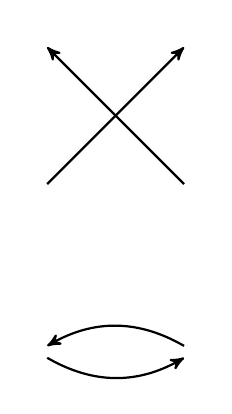
\begin{tikzpicture}[->,>=stealth',auto,node distance=3cm,
  thick,main node/.style={circle,draw,font=\sffamily\Large\bfseries}]
					\node (TU) at (0,0) {};
					\node (UT) at (2,0) {};
					\node (TUexit) at (0,2) {};
					\node (UTexit) at (2,2) {};
					\node (TUend) at (0,4) {};
					\node (UTend) at (2,4) {};
				\path[every node/.style={font=\sffamily\small}]
					(TU) edge[bend right] node {} (UT)
					(UT) edge[bend right] node {} (TU)
					(TUexit) edge node {} (UTend)
					(UTexit) edge node {} (TUend);
\end{tikzpicture}
			}
		\end{minipage}
	\begin{minipage}[r][10cm][t]{.4\textwidth}
			\begin{minipage}[t]{\textwidth}
\begin{lstlisting}
// Specialized Template
// N_U == S_U
// N_T == S_T
template <int S_U,int S_T>
struct UT<S_U,S_T,S_U,S_T> {
	static void split(
	   array<float,S_U>& w_U,
	   array<float,S_T>& w_T,
		 float dt)
	{ /* terminate */ }
};
\end{lstlisting}
			\end{minipage} \\
			\vspace{5mm}
			\begin{minipage}[t]{\textwidth}
\begin{lstlisting}
template <int N_U,int N_T,
           int S_U,int S_T>
struct UT {
	static void split(
	  array<float,S_U>& w_U,
	  array<float,S_T>& w_T,
		float dt)
		/* U */
		stepU(w_U(N_U)*dt);
		/* TU... */
		TU<N_T,N_U+1,S_T,S_U>
		   ::split(w_T,w_U,dt);
	}
};
\end{lstlisting}
			\end{minipage}
	\end{minipage}
	\end{minipage}
	\caption{Simplified C++ snippets for outlining the template invocation sequence in the \proc{IntSplit} function. The template parameters \proc{S\_T} and \proc{S\_U} denote the total size of the coefficient arrays \proc{w\_T} and \proc{w\_U} while the \proc{N\_T} and \proc{N\_U} are the indices of the current coefficient to be applied. The \proc{TU::split} and \proc{UT::split} methods first apply their own step and then invoke each other by gradually incrementing the indices \proc{N\_T} and \proc{N\_U}. \\
	When the conditions \proc{N\_T == S\_T} and \proc{N\_U == S\_U} are satisfied, the partially specialized templates become active and the recursion is terminated.}
	\label{fig:intsplit}
\end{figure}


\subsection{Static Polymorphism through CRTP and enable\_if}
\label{subsec:poly}
inheritance: ugly implementational details are hidden in base class Propagators.
This was achieved by introducing a class hierarchy for the propagators, meaning that all 
\cite{C_CRTP}

Allows to implement the basic building blocks in a generic but efficient manner.




\clearpage
\section{Benchmark / Case Study / Example}

IDEA: express cost of every propagator as a ratio to the hagedorn propagator

\clearpage
\section{Conclusion}

% TODO: final observations
% TODO: suggestions for future work














%%%%%%%%%%%%%%%%%%%%%%%%%%%%%%%%%%%%%%%%%%%%%%%%%%%%%%%%%%%%%%%%%%%%%%%%%%%%%%%%%%%%%
%%%%%%%%%%%%%%%%%%%%%%%%%%%%%%%%%%%%%%%%%%%%%%%%%%%%%%%%%%%%%%%%%%%%%%%%%%%%%%%%%%%%%
%%%%%%%%%%%%%%%%%%%%%%%%%%%%%%%%%%%%%%%%%%%%%%%%%%%%%%%%%%%%%%%%%%%%%%%%%%%%%%%%%%%%%































\clearemptydoublepage

\appendix
% \input{./deriv_ew.tex}
% \input{./color_code.tex}
% \input{./ack.tex}

\clearemptydoublepage

\bibliographystyle{plain}
\bibliography{references,mt,bt,chem,wp,own,propagators}

\end{document}
